\section{Tabela assíncrona (JTable)}

Nesta seção veremos como implementar uma tabela \texttt{assíncrona}
(\texttt{JTable}) usando o \texttt{MDArte}. Para tal, vamos considerar como
ponto de partida o modelo do caso de uso \texttt{Consulta Estudante} conforme as
alterações feitas no tópico anterior. Certifique-se de ter removido o
estereótipo \texttt{«Manageable»} da classe \texttt{Estudante} no diagrama de
classes que descreve a \texttt{Camada de domínio}, a fim de evitar que o
\texttt{CRUD} seja re-gerado, sobrescrevendo assim as alterações que faremos.

Veremos agora, por subseções, algumas das funcionalidades disponíveis na tabela
assíncrona.

\subsection{Implementando filtragem assíncrona da tabela}
Nesta seção veremos como criar uma action ajax que reflita nos dados exibidos
por uma tabela ajax. A título de exemplo, faremos uma tela com um formulário e
um botão que, uma vez clicado, recarregará a tabela filtrando-a de acordo com os
dados do formulário. Tomaremos como base a tabela criada no exemplo de criação
de tabelas.

O modelo portanto começará assim:

\begin{figure}[H]
	\centering
	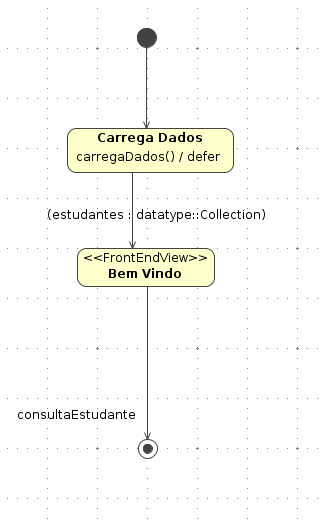
\includegraphics[width=180pt,height=260pt]{files/imgs/tutorial-mdarte-0040.png}
	\caption{Modelagem da filtragem assíncrona da tabela.}
	\label{modelando_filtragem_assincrona}
\end{figure}

Modelaremos então uma \texttt{transition} saindo da \texttt{FrontEndView} que
contém a nossa tabela e retornando para a mesma \texttt{view}, que será
interpretada pelo \texttt{MDArte} como uma ação assíncrona na \texttt{view}.
Abriremos então sua especificação e iremos na aba \texttt{tagged values} e
selecionaremos o \texttt{tagged value}
\texttt{@andromda.presentation.web.action.async.table} e daremos a ele o valor
\texttt{[nome-da-tabela]} (\texttt{estudantes}, nesse caso), esse \texttt{tagged
value} indica qual tabela será afetada pela ação assíncrona, nos permitindo ter
mais de uma de tabela assíncrona na mesma tela, tendo \texttt{actions} que
afetem somente uma tabela sem afetar a outra. Iremos então na aba
\texttt{general} e clicaremos no botão \texttt{edit} no \texttt{fieldset}
\texttt{'trigger'}, daremos o nome que desejarmos o \texttt{trigger} criado, no
exemplo fo idado o nome de \texttt{“filtrar”}, e selecionaremos seu tipo como
\texttt{signal}. Iremos então na aba \texttt{parameters}, ainda na especificação
do \texttt{trigger} e criaremos os parâmetros necessários para o processamento
da requisição, neste exemplo colocaremos só os parâmetros \texttt{matrícula} e
\texttt{nome}, a título de ilustração, e definiremos seus tipos como
\texttt{String}.

O modelo ficará assim:
\begin{figure}[H]
	\centering
	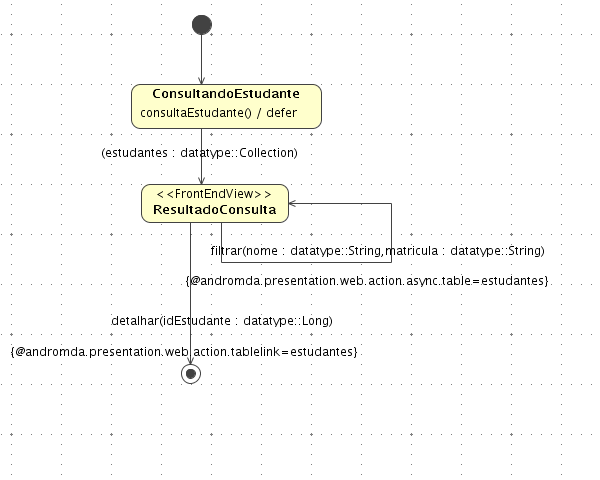
\includegraphics[width=340pt,height=300pt]{files/imgs/tutorial-mdarte-0036.png}
	\caption{Modelagem da filtragem assíncrona da tabela.}
	\label{modelando_filtragem_assincrona}
\end{figure}

Executaremos agora o seguinte comando para validar o modelo e regerar o
sistema:
\begin{lstlisting}[language=bash, frame=single, breaklines=true]
maven mda -Dprojeto=sistemaacademico-geral-Estudante
\end{lstlisting}

Agora adaptaremos, no \texttt{ControleImpl}, os métodos responsáveis pelo
carregamento da tabela, com a assinatura \texttt{public final Collection
load[nome-da-view][nome-da-tabela]Table}, e pelo retorno do número máximo de
elementos na mesma, com a assinatura \texttt{public final Integer
get[nome-da-view][nome-da-tabela]TableLength}, a fim de implementarmos o filtro.
Cada parâmetro da \texttt{trigger} pertencente à \texttt{transition} modelada
será adicionado, em ordem, à lista de parâmetros de cada método, logo antes do
parâmetro \texttt{ViewContainer container}. De acordo com o nosso exemplo, o
código ficará assim:
\lstinputlisting[language=java, frame=single, breaklines=true]{files/java/JTableFiltro.java}

Executaremos agora o seguinte comando para compilar e dar \texttt{deploy} no
sistema:
\begin{lstlisting}[language=bash, frame=single, breaklines=true]
maven compile deploy
\end{lstlisting}

Restartando o servidor e abrindo o caso de uso \texttt{Consulta Estudante},
veremos o resultado do que fizemos:
\begin{figure}[H]
	\centering
	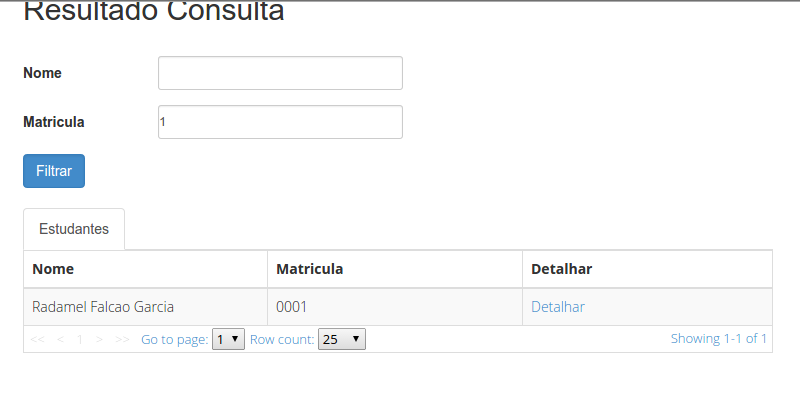
\includegraphics[width=340pt,height=300pt]{files/imgs/tutorial-mdarte-0042.png}
	\caption{Modelagem da filtragem assíncrona da tabela.}
	\label{modelando_filtragem_assincrona}
\end{figure}
